\chapter{Software}
\label{cha:software}

Oprogramowanie słuchawek zostało napisane w języku C z wykorzystaniem bibliotek HAL, które zawierają dużo gotowych funkcji, na przykład do uruchomienia timera lub do odczytu wartości z przetwornika. Użyto narzędzia \textit{System Workbench for STM32}, które jest zbudowane na popularnym IDE \textit{Eclipse}. Dodatkowo kod do konfiguracji i inicjalizacji peryferiów został wygenerowany z użyciem \textit{CubeMX}.

Tak jak przy pozostałych elementach projektu, wykorzystano repozytorium do zapisywania postępów: \url{https://github.com/Hoplophile/TacticalHeadphones_SW.git}

\begin{figure}[H]
	\centering
	\begin{subfigure}{.48\textwidth}
		\centering
		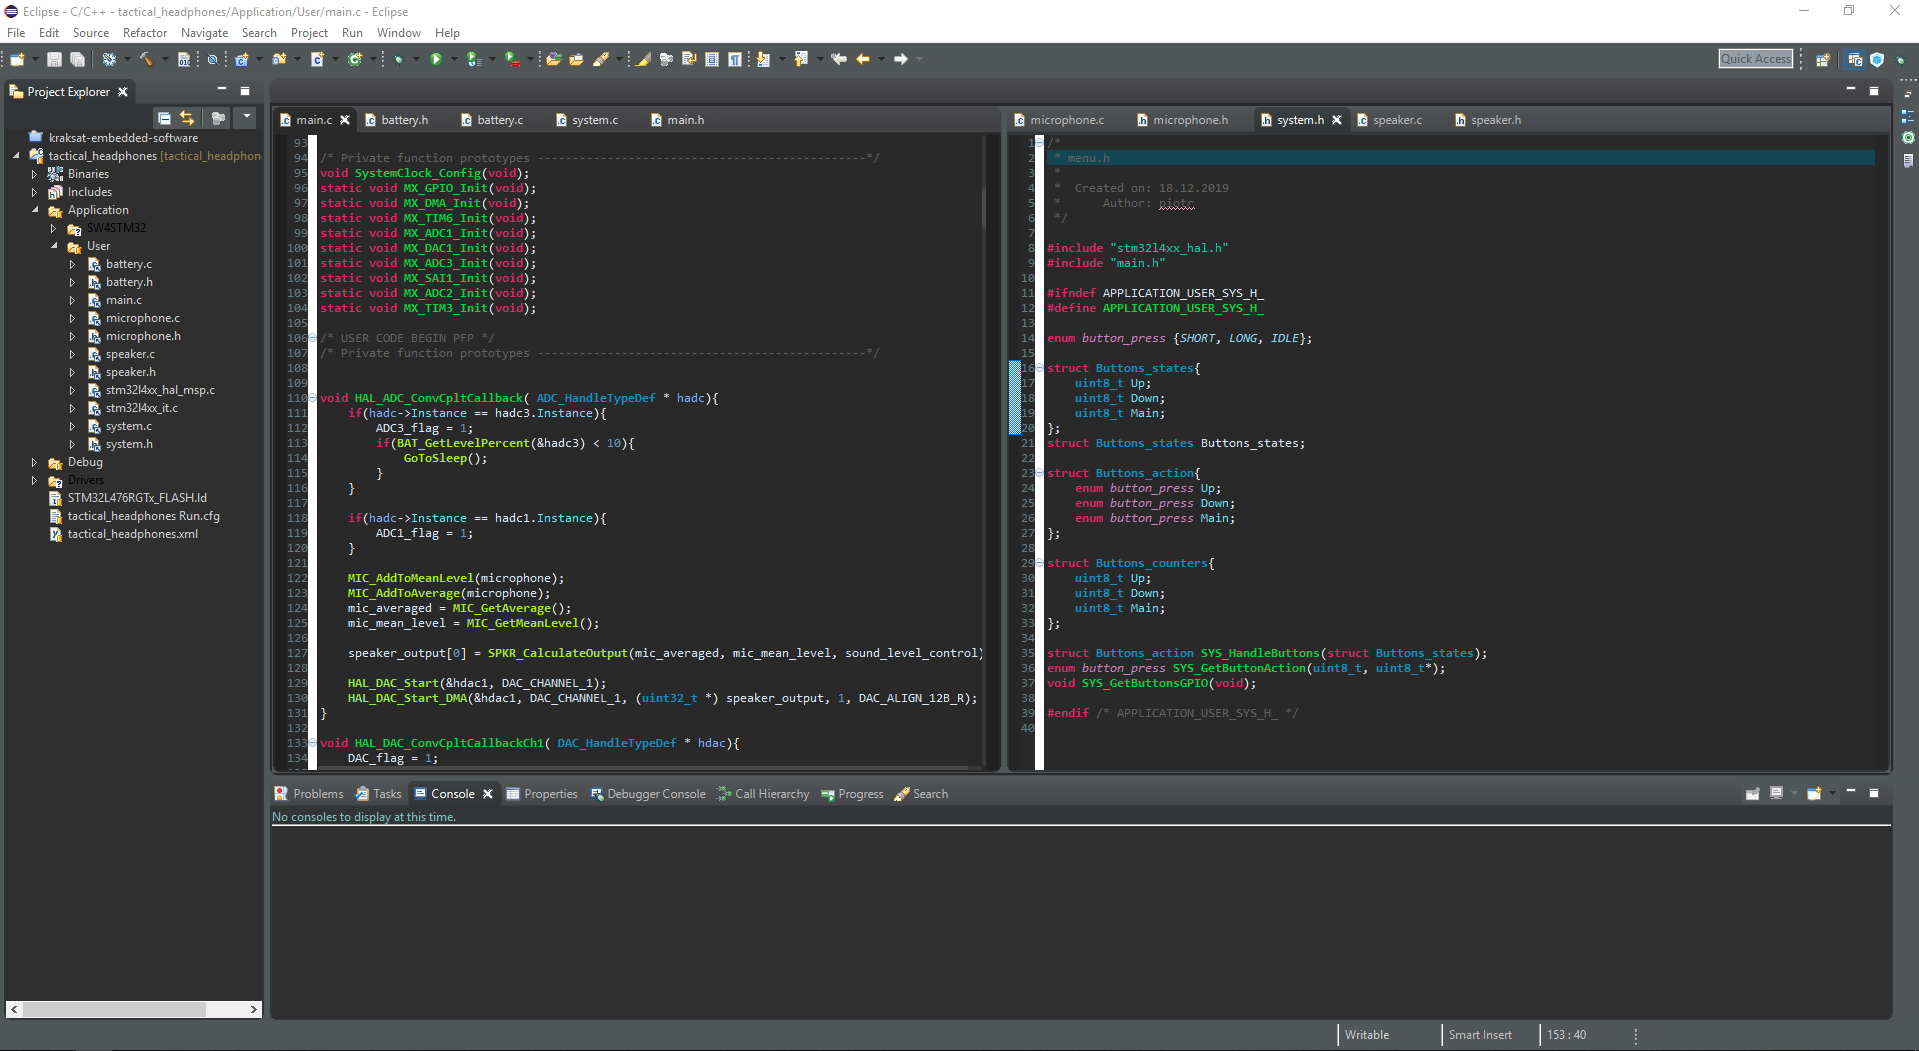
\includegraphics[height=4.2cm]{zdjecia/eclipse.png}
		\subcaption{System Workbench for STM32}
	\end{subfigure}
	\begin{subfigure}{.48\textwidth}
		\centering
		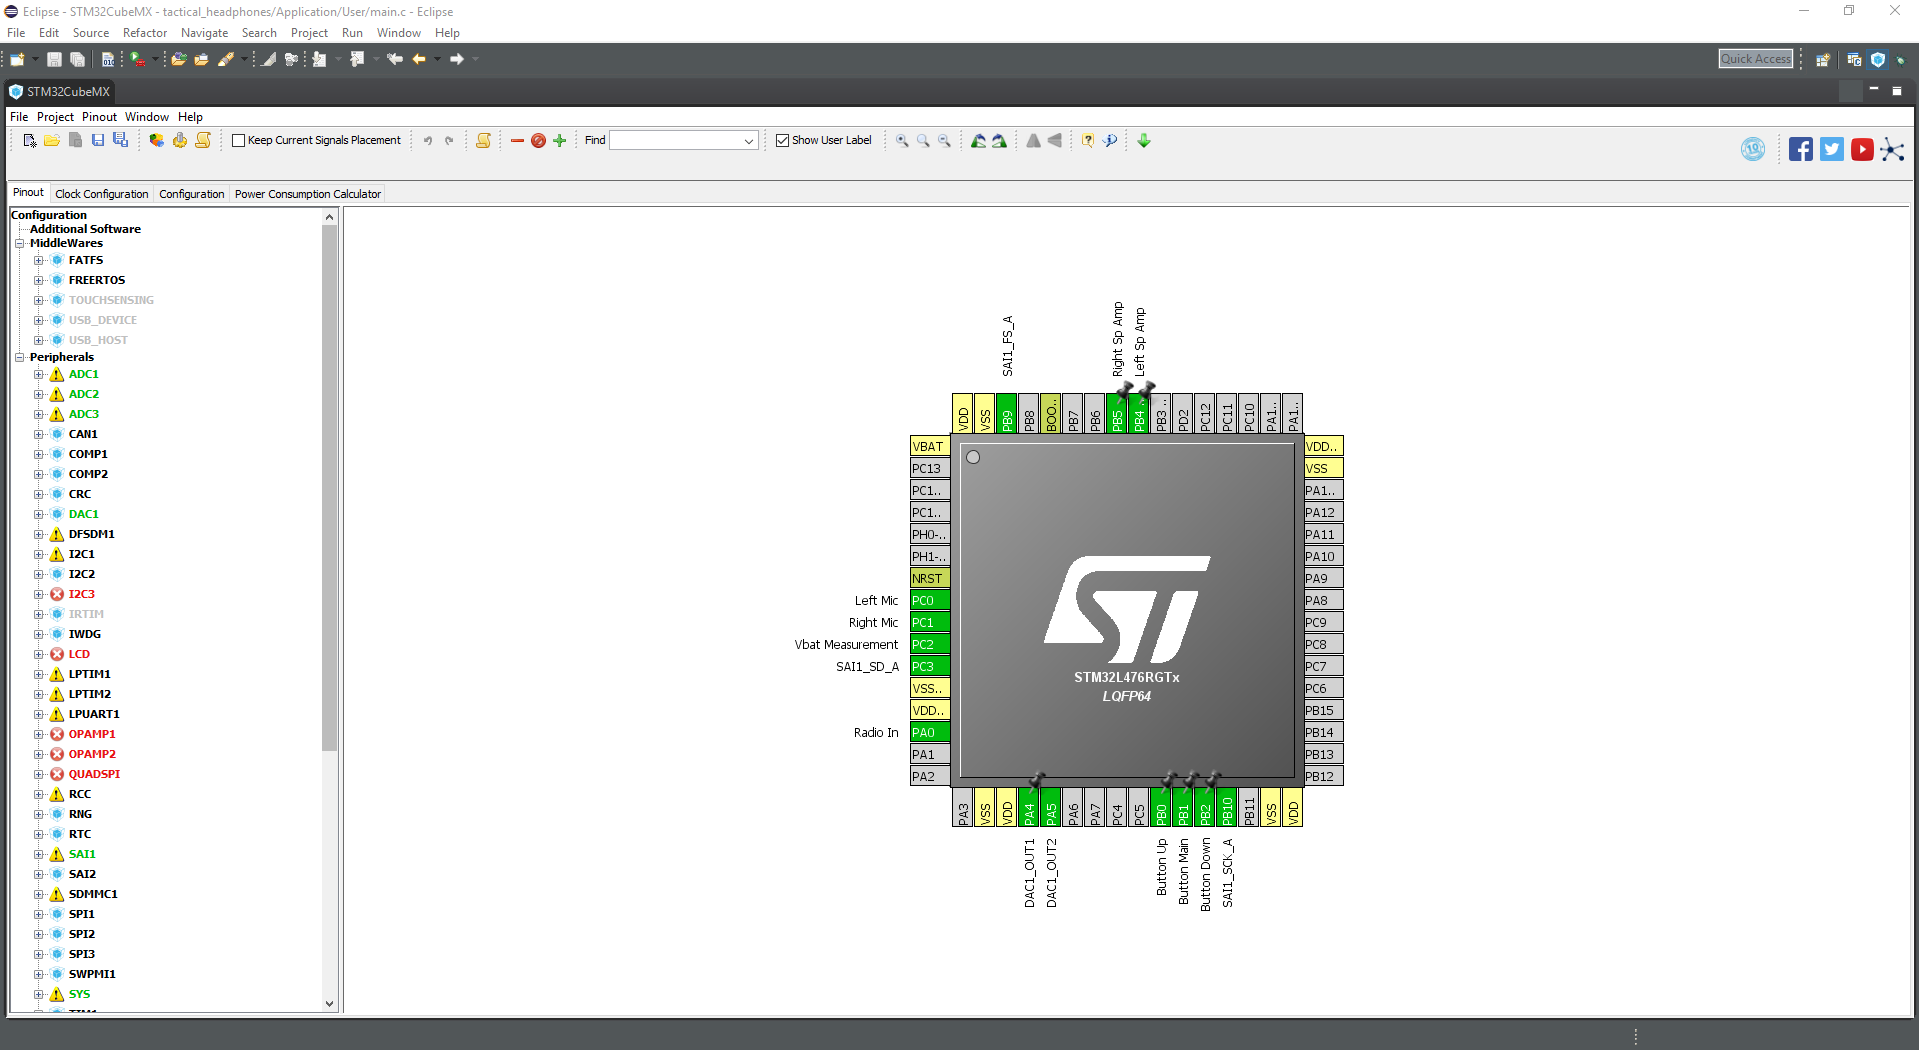
\includegraphics[height=4.2cm]{zdjecia/cubemx.png}
		\subcaption{CubeMX}
	\end{subfigure}
	\caption{\label{pic:IDE} Środowiska użyte do rozwoju oprogramowania}
\end{figure}

Kod był pisany tak, aby rozdzielić program na funkcje wykonujące niewielkie fragmenty. Przewidziano także elastyczną możliwość modyfikacji lub dodawania funkcjonalności, na przykład implementując do $V_{BAT}$ 3 funkcje, odczytujące kolejno: wartość surową, przeliczoną na Volty oraz procenty naładowania. W obecnej wersji użyta została ta ostatnia.

Dla lepszej nawigacji, zastosowano konwencję nazewnictwa funkcji - <NAZWA\_ZWIĄZANA\_Z\_NAZWĄ\_PLIKU>\_<funkcjonalnośćFunkcji>. Na przykład funkcja dodająca wartość do średniego poziomu sygnału mikrofonu zawarta w pliku \textit{microphone.c} została nazwana \textit{MIC\_AddToMeanLevel}.